\indent\underline{\textbf{Ejercicio 5}}\\
\textcolor{green}{[Programación]} Implemente el Algoritmo de Iteración de Valores para el el Ejemplo 4.3 (\textit{Gambler’s problem, Sutton\&Barto, 2018})~\cite{Sutton2018} para los siguientes casos:

\begin{itemize}
    \item $p_h = 0.25$.
    \item $p_h = 0.55$.
\end{itemize}

\indent\underline{\textbf{Solución}}\\
La implementación de los algoritmos se realizó en Python, que se puede encontrar en el repositorio de \href{https://github.com/MasterUBA-DM-KD/Aprendizaje_Reforzado/blob/5ae50da937b14f0a11c416e40019a4b5661dd51b/docs/guia/3/notebooks/utils.py}{GitHub}.

Sea,\\
$N=100$: capital máximo\\
$S=\left\{0, 1, \ldots, 100\right\}$: conjunto de estados\\
$A=\left\{0, 1, \ldots, \min(s, 100-s)\right\}$: conjunto de acciones\\

El Algoritmo de Iteración de Valores para el Ejemplo 4.3 (\textit{Gambler’s problem, Sutton\&Barto, 2018})~\cite{Sutton2018} se implementó en Python\footnotemark.
A continuación, los resultados de la implementación, $p_h = 0.25$, se muestran en las figuras~\ref{fig:ph_025_sweeps} y~\ref{fig:ph_025_policy}.

\footnotetext{Se fijó una tolerancia de $10^{-3}$ para la convergencia.}

\begin{figure}[H]
    \centering
    \begin{subfigure}[H]{0.45\textwidth}
        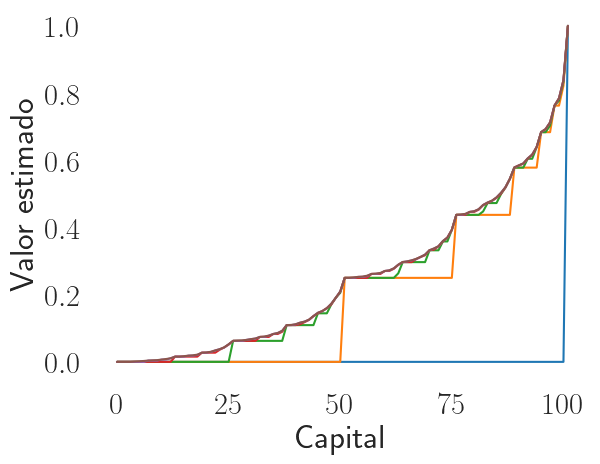
\includegraphics[width=\textwidth]{../img/sweeps_0.25}
        \caption{$sweeps \in [0, N]$}
        \label{fig:ph_025_sweeps}
    \end{subfigure}
    \begin{subfigure}[H]{0.45\textwidth}
        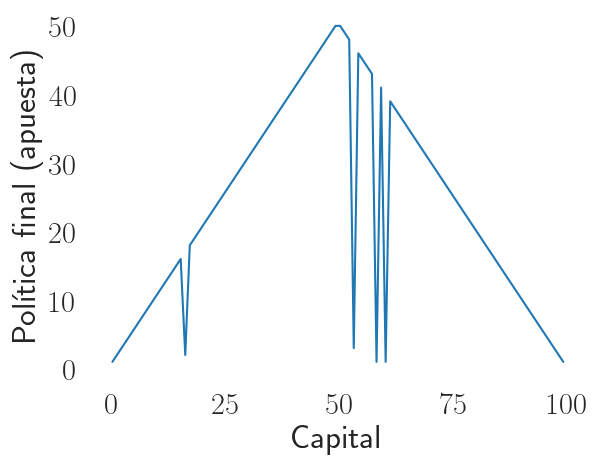
\includegraphics[width=\textwidth]{../img/policy_0.25}
        \caption{Política final}
        \label{fig:ph_025_policy}
    \end{subfigure}
    \caption{$ph=0.25$}
    \label{fig:ph_025_gamblers_problem}
\end{figure}

A continuación, los resultados de la implementación, $p_h = 0.55$, se muestran en las figuras~\ref{fig:ph_055_sweeps} y~\ref{fig:ph_055_policy}.

\begin{figure}[H]
    \centering
    \begin{subfigure}[H]{0.45\textwidth}
        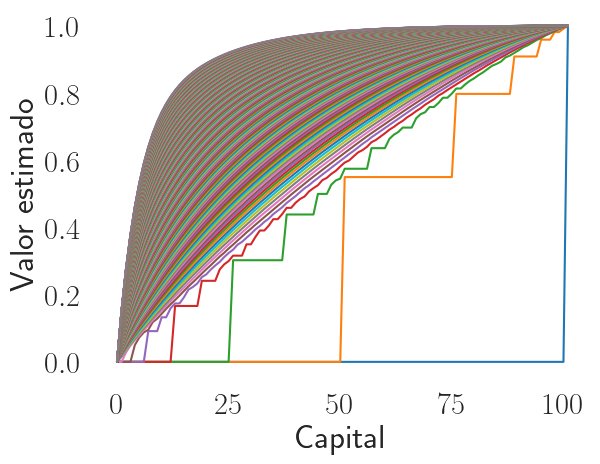
\includegraphics[width=\textwidth]{../img/sweeps_0.55}
        \caption{$sweeps \in [0, N]$}
        \label{fig:ph_055_sweeps}
    \end{subfigure}
    \begin{subfigure}[H]{0.45\textwidth}
        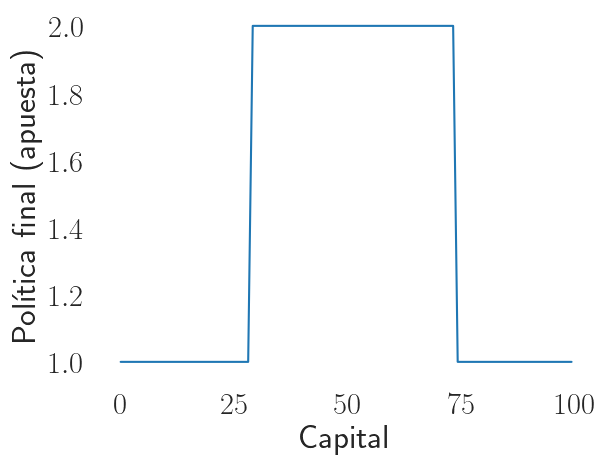
\includegraphics[width=\textwidth]{../img/policy_0.55}
        \caption{Política final}
        \label{fig:ph_055_policy}
    \end{subfigure}
    \caption{$ph=0.55$}
    \label{fig:ph_055_gamblers_problem}
\end{figure}

\indent\underline{\textbf{Conclusiones}}
\paragraph{Convergencia} En las figuras~\ref{fig:ph_025_sweeps} y~\ref{fig:ph_055_sweeps} se muestra que a medida que se aumentan las iteraciones (sweeps), los valores de vada estado convergen a un valor estable.

\paragraph{Política final} Se encuentra influenciada por el valor de $p_h$.
Cuando la probabilidad de ganar es baja la política óptima es apostar poco, especialmente cuando el capital es bajo, hecho que se deba al alto riesgo de perder el capital.
Además, para este caso la política final tiene forma de \textit{V} invertida como se muestra en la figura~\ref{fig:ph_025_policy}.

Por otro lado, cuando la probabilidad de ganar es alta, la política óptima es apostar más, especialmente cuando el capital es intermedio, hecho que se debe a la alta probabilidad de ganar y la posibilidad de maximizar la ganancia.
Además, para este caso la política final tiene forma de \textit{V} achatada, como se muestra en la figura~\ref{fig:ph_055_policy}.

En ambos casos:
\begin{itemize}
    \item Se apuesta poco si se tiene poco capital para evitar perderlo.
    \item Se apuesta más si se tiene un capital intermedio, aprovechando la oportunidad de ganar.
    \item Se apuesta poco si se tiene mucho capital para asegurar ganancia.
\end{itemize}

Se hace la salvedad que en el caso de $p_h = 0.25$ la política final tiene un máximo en el que se encuentra poca estabilidad.

\line(1,0){\textwidth}
